\subsection{Modèle statistique pour l'alignement des séquences}

Pour comparer de plus en plus de génomes, de nouvelles méthodes vont s'appuyer sur la modélisation statistique des séquences pour améliorer les performances de l'alignement et aligner de grands jeux de données. Chaque modèle représentera un ensemble de séquences et établit une fréquence ou probabilité d'un résidu pour chaque position. Ce modèle peut être assimilé à une séquence "consensus" du groupe.

\subsubsection{Partitionnement des séquences par similarité. }
\label{sec:clustering}

Les méthodes de partitionnement, ou \textit{clustering} en anglais, reposent sur les méthodes d'alignement pour déterminer la similarité des séquences, et les graphes pour représenter les liens de similarité entre chaque séquence. 

De manière générale, on va regrouper les séquences en groupes d'homologues en utilisant un seuil de similarité plus ou moins élevé. Les outils sont régulièrement présentés en utilisant la séquence protéique plutôt que nucléique pour calculer la similarité. Ce choix permet de réduire la complexité tout en étant plus précis sur l'évaluation de la similarité fonctionnelle et structurelle, mais aussi d'identifier des homologies plus lointaines. Dans ce cas, il faudra faire attention à la nuance entre similarité et identité. Ce qui va varier entre les méthodes, c'est l'algorithme de partitionnement utilisé. Le \autoref{tab:clustering} présente un aperçu des méthodes et des outils existants.  

\begin{table}[htbp]
    \footnotesize
    \centering
    \begin{tabular}{|p{0.2\textwidth}|p{0.25\textwidth}|p{0.25\textwidth}|p{0.25\textwidth}|}
\hline
\textbf{Outil} & \textbf{Description} & \textbf{Avantages} & \textbf{Inconvénients} \\
\hline
COGs \cite{tatusov_genomic_1997} & Classification basée sur l'évolution. Les clusters obtenus sont des groupes de protéines orthologues & Base de données bien documentées et largement utilisée & Méthode statique, mise à jour peu fréquente. \\
\hline
CD-HIT \cite{li_clustering_2001} & Clustering rapide basé sur la longueur des séquences, en ordonnant les protéines de la plus longue à la plus courte & Très rapide et efficace pour réduire la redondance & Sensibilité limitée pour les faibles identités de séquence \\
\hline
InParanoid \cite{remm_automatic_2001} & Détection des orthologues et paralogues en comparant deux génomes & Fiable pour détecter des orthologues proches, distingue bien orthologues et paralogues & Moins adapté aux comparaisons multi-génomes \\
\hline
OrthoMCL \cite{li_orthomcl_2003} & Identification des orthologues et paralogues récents via une approche basée sur les graphes & Bonne précision, adaptable à divers organismes & Consommation élevée en ressources pour les grands ensembles de données \\
\hline
UCLUST \cite{edgar_search_2010} & Alignement et clustering rapide des séquences protéiques & Très rapide, faible consommation mémoire & Moins précis que BLAST pour certaines comparaisons \\
\hline
Proteinortho \cite{lechner_proteinortho_2011} & Détection rapide d'orthologues à grande échelle & Évolutif et performant pour l'analyse de nombreux génomes & Moins détaillé sur les relations fonctionnelles des protéines \\
\hline
BUSCO \cite{simao_busco_2015} & Évaluation de la complétude des génomes en utilisant des ensembles de gènes conservés & Référence fiable pour les génomes récemment séquencés & Ne permet pas une recherche extensive d'orthologues \\
\hline
OMA \cite{altenhoff_oma_2019} & Méthode évolutive d'identification des orthologues & Haute précision sur les génomes bien annotés & Temps de calcul élevé pour les grands jeux de données \\
\hline
SwiftOrtho \cite{hu_swiftortho_2019} & Similaire à OrthoMCL, utilisant des k-mers longs pour améliorer la rapidité & Très rapide et nécessite peu de ressources & Peut être moins précis pour des génomes très divergents \\
\hline
SonicParanoid \cite{cosentino_sonicparanoid_2019} & Extension de InParanoid pour la détection rapide d'orthologues & Améliore la vitesse et réduit les besoins en ressources & Moins précis pour des génomes très distants évolutivement \\
\hline
OrthoFinder \cite{emms_orthofinder_2019} & Détection des orthologues basée sur une approche évolutive & Haute précision grâce à l'utilisation de scores de similarité normalisés & Temps de calcul élevé pour les grands ensembles de données \\
\hline
OrthoPhy \cite{watanabe_orthophy_2023} & Intègre les informations taxonomiques dans l'identification des orthologues & Minimise les erreurs de prédiction et améliore la fiabilité & Exige davantage de ressources et est plus lent sur de grandes bases de données \\
\hline
\end{tabular}
\caption[Outils de clustering des séquences]{\textbf{Présentation des principaux  outils de clustering de séquences avec leurs descriptions, avantages et inconvénients.}}
\label{tab:clustering}
\end{table}

\newpage
\subsubsection{MMSeqs2}

Un outil largement utilisé pour l'alignement et le \textit{clustering} de grand jeu de données est l'outil MMSeqs2 \cite{steinegger_mmseqs2_2017}. L'objectif de MMSeqs2 est de partitionner les séquences en groupes d'homologues, de manière rapide et efficace. MMSeqs2 s'appuie sur les technologies informatiques, tant matérielles que logicielles, pour optimiser les ressources utilisées, et sur un nouvel algorithme de recherche de k-mer similaire. 

MMSeqs2 ne va pas faire des comparaisons exactes de k-mers, mais il va chercher des k-mers similaires. Cette différence permet de comparer les k-mers plus rapidement tout en utilisant des k-mers de plus grandes tailles, améliorant sa sensibilité\footnote{La sensibilité correspond au nombre de séquences qui sont alignées par rapport au nombre de séquences qui sont similaires.}. Comme présenté sur la \autoref{fig:mmseqs2}, les k-mers utilisés sont "espacés", ce qui permet un recouvrement plus important de la séquence et donc de réduire les alignements liés au hasard de k-mers successifs entre 2 séquences non homologues. S'appuyant sur cette caractéristique, les auteurs de MMSeqs2 vont supposer que si les séquences ont des k-mers similaires, séparé par le même nombre de résidus, alors la zone entre les k-mers à des chances de s'aligner, ce qui permet d'étendre les zones alignables (diagonale). Enfin, un score associé aux diagonales va être utilisé pour filtrer les séquences qui ont le plus de probabilités de s'aligner.

\begin{figure}[htbp]
    \centering
    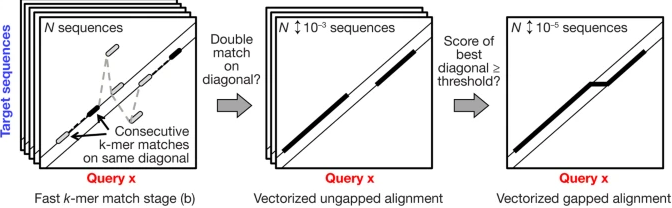
\includegraphics[width=\textwidth]{images/mmseqs2.png}
    \caption[Principe de l'alignement de MMSeqs2.]{\textbf{Principe de l'alignement de MMSeqs2.}  Extrait de \cite{steinegger_mmseqs2_2017}}
    \label{fig:mmseqs2}
\end{figure}

Une fois l'étape d'alignement terminée, MMSeqs2 intègre plusieurs algorithmes pour partitionner les séquences. Dans chacun de ces algorithmes, chaque groupe de séquences similaires (partie) verra une des séquences (n\oe ud) utilisée comme référente. (\textit{i}) L'algorithme Set-cover (\autoref{fig:set-cover}) sélectionne le n\oe ud avec le plus d'arêtes comme référent et forme une partie avec tous les n\oe uds dans un voisinage direct, puis de manière itérative reproduit le schéma jusqu'à ce que tous les n\oe uds soient dans une partie. (\textit{ii}) L'algorithme \textit{Connected Component} (\autoref{fig:connected-componet}) fonctionne comme Set-cover, mais partitionne tous les n\oe uds pour lesquels il existe un chemin avec le n\oe ud référent. (\textit{iii})  l'algorithme \textit{CD-hit like} (\autoref{fig:cdhit}) prend pour référence le n\oe ud dont le poids (taille de la séquence) est le plus élevé, puis forme une partie avec tous les voisins directs. Ces algorithmes répondent chacun à des problématiques différentes que nous pourrons illustrer dans la suite.  

\begin{figure}[htbp]
    \centering
    \subfloat[Set-cover]{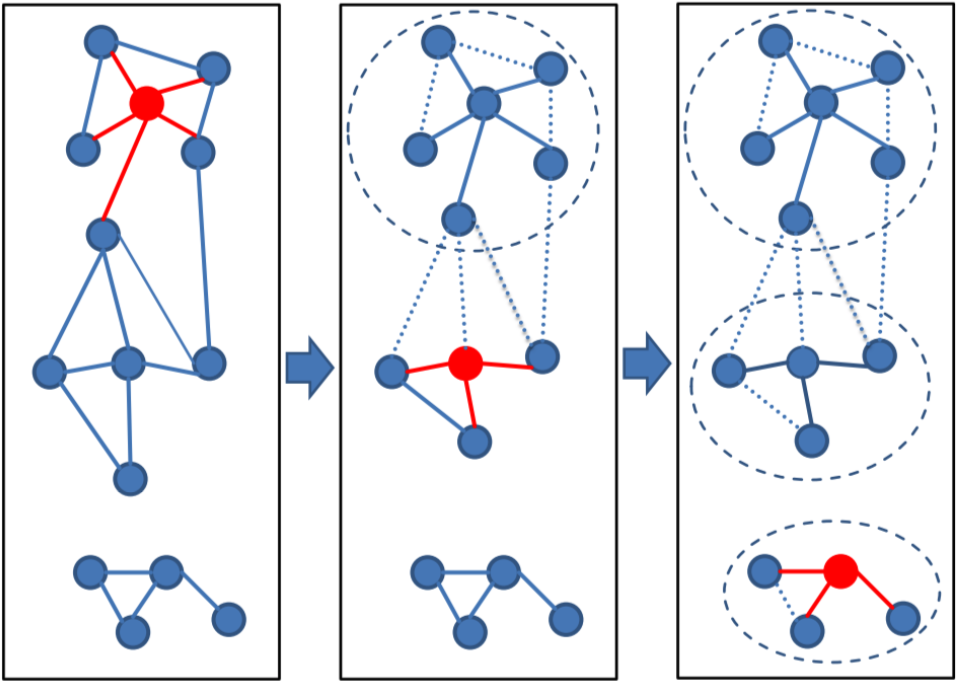
\includegraphics[width=.3\textwidth]{images/cluster-mode-setcover.png}
    \label{fig:set-cover}}
    \hfill
    \subfloat[Connected component]{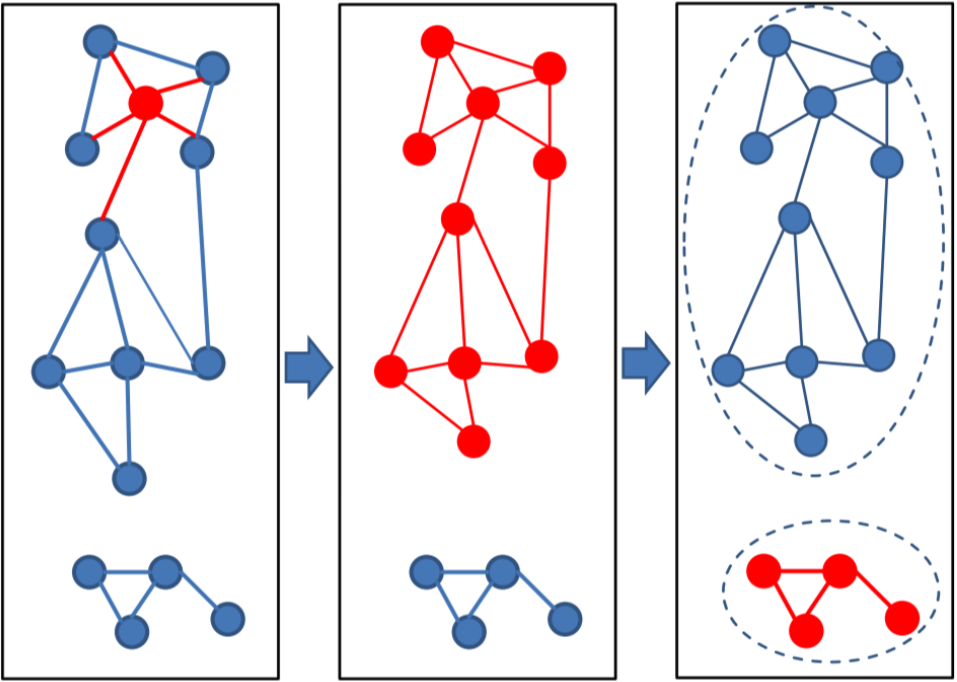
\includegraphics[width=.3\textwidth]{images/cluster-mode-connectedcomp.png}
    \label{fig:connected-componet}}
    \hfill
    \subfloat[CD-hit like]{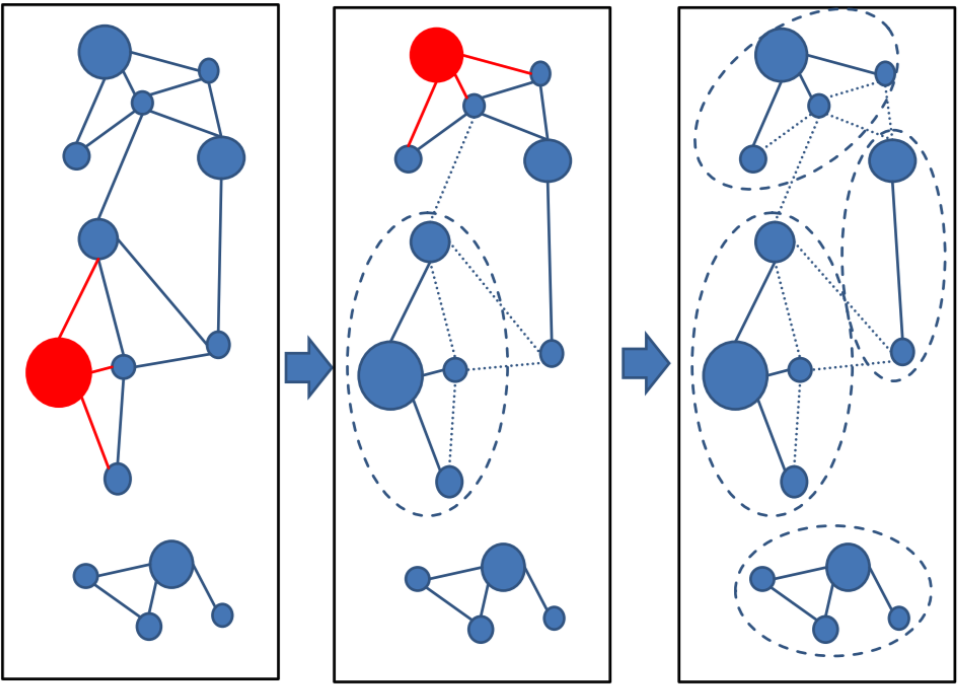
\includegraphics[width=.3\textwidth]{images/cluster-mode-greedyincremental.png}
    \label{fig:cdhit}}
    \caption[Algorithmes de clustering de MMSeqs2]{\textbf{Les algorithmes de clustering de MMSeqs2.}}
    \label{fig:mmclust}
\end{figure}

\newpage

Depuis 2018, MMSeqs2 intègre une nouvelle méthode appelée Linclust \cite{steinegger_clustering_2018}. Celle-ci vise à proposer un clustering dont la durée évolue linéairement avec le nombre de séquences. Pour ce faire, les séquences ne sont pas alignées entre elles. Dans un graphe, chaque séquence forme un n\oe ud et est représentée par des k-mers, eux-mêmes répartis en groupes. La séquence la plus longue de chaque groupe est comparée à toutes les autres. Si l'alignement dépasse un seuil prédéfini, une arête de similarité est établie entre les séquences. Ensuite, un algorithme de partitionnement est appliqué au graphe résultant pour obtenir le partitionnement final. Cette optimisation permet de partitionner rapidement de grands jeux de données.

\subsubsection{Modélisation des séquences similaires : matrices de position, profils et chaînes de Markov}

Une fois les séquences regroupées par similarité, il est possible de créer un modèle statistique représentant les séquences, sous forme de "séquence" consensus. L'idée générale de ces modèles va être, pour chaque position de la séquence consensus, d'associer pour chaque type de résidus une fréquence ou probabilité d'apparition, basée sur un alignement multiple des séquences.

Les premiers modèles statistiques correspondaient à des matrices de score à position spécifique (PSSM, position-specific scoring matrices), représentant la probabilité du résidu à une position donnée. Ainsi la matrice obtenue reflète pour un score positif une correspondance de résidus similaires parmi les séquences, ou pour un score négatif un résidu non conservé. Ces matrices ont été utilisées dans des outils comme CLUSTAL \cite{higgins_clustal_1988} ou MATCH$^{TM}$ \cite{kel_matchtm_2003} pour la recherche de facteur de transcription dans les séquences d'ADN, ou encore dans l'algorithme ESAsearch \cite{beckstette_fast_2006} pour rechercher des séquences dans les PSSMs. Ces outils vont également amener une variante aux PSSMs qui comble un défaut de ces dernières. En effet, le score dépend du nombre et de la divergence des séquences utilisées dans le MSA. Si la matrice est constituée de peu de séquences ou si des séquences proches sont surreprésentées, alors le score sera biaisé. C'est pourquoi un poids est appliqué pour réduire l'impact des séquences proches et augmenter celui des séquences divergentes. 

Pour construire une PSSM, les MSA doivent être continus (sans \textit{gap}), ce qui est rarement le cas. Une nouvelle forme de PSSM, appelée profil, va prendre en compte les \textit{gap} en appliquant des pénalités. Un profil est donc une PSSM intégrant les possibles indels sous forme de pénalités\footnote{Dans la littérature, les PSSM sont souvent également appelées profils.}. Les profils sont utilisés, notamment dans le contexte des bases de données, pour rechercher des séquences homologues à un groupe de séquences sans aligner chacune des séquences du groupe. PSI-BLAST \cite{altschul_gapped_1997}, développé par les auteurs de BLAST, permet de construire des profils et de rechercher des séquences contre un profil. Bien que PSI-BLAST soit reconnu pour sa haute précision, il demeure sensible aux erreurs d'assignation initiales, lesquelles peuvent introduire des biais dans les profils générés et impacter la fiabilité des cycles et des itérations suivants.

Une dernière forme de modèle s'appuie sur les chaînes de Markov cachées (\textit{Hidden Markov Model} en anglais, HMMs). Une chaîne de Markov décrit la probabilité de transition vers un état en fonction des états précédents. Dans nos modèles, cela correspondrait à calculer la probabilité d'un résidu (état) à une position donnée en fonction des résidus des positions précédentes. Une chaîne de Markov cachée inclut, en plus, l'existence de facteurs non observables sur la probabilité de transition. Dans nos modèles, ces facteurs cachés peuvent être les \textit{gaps} qui ne correspondent à aucun résidu (état) mais influencent la probabilité de transition (\autoref{fig:HMM_ex}). On peut alors obtenir une probabilité pour chaque résidu à chaque position. 

\begin{figure}[htbp]
    \centering
    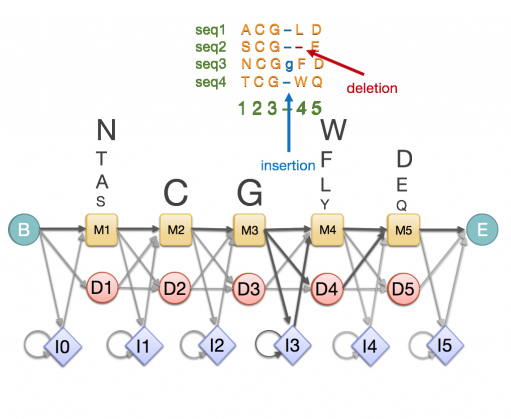
\includegraphics[width=0.5\linewidth]{images/HMM_ex.png}
    \caption[Exemple de modélisation HMM d'une séquence]{\textbf{Exemple de modélisation HMM d'une séquence.} Les cases jaunes représentent les états de correspondance (M), où la distribution de probabilité est déterminée par la fréquence des acides aminés à cette position. La rangée d'états en forme de losange correspond aux états d'insertion (I) et les états circulaires désignent les états de suppression (D). Ce modèle probabiliste permet d’estimer les fréquences observées des acides aminés à chaque position et de représenter les transitions entre eux, sur la base de l’occupation observée des positions dans un alignement de séquences multiples. Extrait de \url{https://www.ebi.ac.uk/training/online/courses/pfam-creating-protein-families/what-are-profile-hidden-markov-models-hmms/}}
    \label{fig:HMM_ex}
\end{figure}

Les modèles HMMs semblent donc tout indiqués pour représenter l'alignement des séquences similaires. Les HMMs, ont l'intérêt de pouvoir différencier les événements d'insertion des événements de délétion par rapport aux profils. Cet avantage les rend plus robustes que les profils. 

Un outil largement utilisé pour construire des HMMs et rechercher des séquences homologues contre une base de données HMMs est HMMER (\url{http://hmmer.org/}). Un autre outil, HH-suite \cite{steinegger_hh-suite3_2019}  intègre la possibilité de faire des comparaisons HMM/HMM. Ces outils, dans leurs versions récentes, ont été optimisés pour combler la complexité sous-jacente de l'utilisation de tels modèles. D'autres outils récents, comme ApHMM \cite{firtina_aphmm_2024} ou le package pyhmmer\cite{larralde_pyhmmer_2023}, proposent des améliorations techniques pour augmenter l'efficacité et la sensibilité des comparaisons aux HMMs, notamment pour ApHMM en s'appuyant sur les nouvelles technologies matérielles et logicielles, et en optimisant les calculs opérés par les algorithmes.

Les modèles HMMs sont couramment utilisés pour la recherche de séquences homologues dans les bases de données. Ils trouvent également des applications dans d'autres domaines, tels que la classification et l'annotation des protéines, ainsi que la prédiction de gènes et de promoteurs \cite{dimri_hidden_2024}.
